\exer{}
\setcounter{numques}{0}

\question{}
\begin{lstlisting}
def reste_a_payer(p,t,m,d):
    """p = montant du pret en euros
       t = taux mensuel
       m = mensualites
       d = duree en annees
       Calcule le montant restant a payer a l'echeance   du pret"""
    dette = p
    for mois in range(d*12):
        # Inv : dette est dû au début du mois
        dette = dette*(1+t)-m
    return dette
 \end{lstlisting}  
    
\question{}    
 
 \begin{lstlisting}   
def somme_totale_payee(p,t,m,d):
    """p = montant du pret
       t = taux
       m = mensualites
       d = duree en annees
       Calcule le montant total paye"""
    return reste_a_payer(p,t,m,d) + 12*d*m
 \end{lstlisting}      
\question{}


\begin{lstlisting}
def cout_total(p,t,m,d):
    """p = montant du pret
       t = taux
       m = mensualites
       d = duree en annees
       Calcule le cout total du credit"""
    return somme_totale_payee(p,t,m,d) - p
\end{lstlisting}

\question{}

\begin{lstlisting}
def duree_mensualite(p,t,m):
    """Durée du prêt
       p = montant prêté
       t = taux mensuel
       m = mensualité"""
    emprunt = p
    d = 0
    while (1+t)*emprunt >= m:
        # Inv : emprunt est dû au début du mois d
        d = d+1
        emprunt = (1+t)*emprunt-m
    return d
\end{lstlisting}

\question{}

Si la mensualité est trop petite la dette augmentera plus vite que le capital restant du diminuera et ainsi la condition de la boucle conditionnelle ne sera jamais vérifiée et la boucle tournera à l'infini.

\question{}

\begin{lstlisting}
import matplotlib.pyplot as plt    
def tracer_mensualite(p,t,m):
    """Trace
       p = montant prêté
       t = taux mensuel
       m = mensualité"""
    emprunt = p
    d = 0
    mois=[]#numero de mensualite
    capital_rd=[]#capital restant du
    interets=[]
    while (1+t)*emprunt >= m:
        # Inv : emprunt est dû au début du mois d
        d = d+1
        emprunt = (1+t)*emprunt-m
        mois.append(d)
        capital_rd.append(emprunt)
        interets.append(t*emprunt)
    plt.clf()
    plt.plot(mois,capital_rd)
    plt.xlabel('Mensualité')
    plt.ylabel('capital restant du')
    plt.savefig('capital_restant_du.png')
    plt.clf()
    plt.plot(mois,interets,'b')
    plt.xlabel('Mensualité')
    plt.ylabel('Intérêts')
    plt.savefig('interets.png')
\end{lstlisting}

\begin{center}
\begin{tabular}{cc}
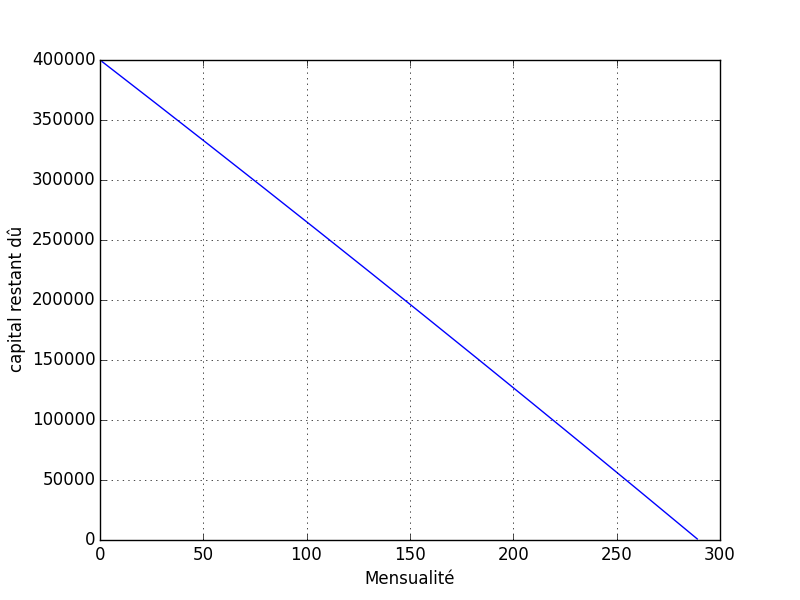
\includegraphics[width=0.5\textwidth]{capital_restant_du.png}
&
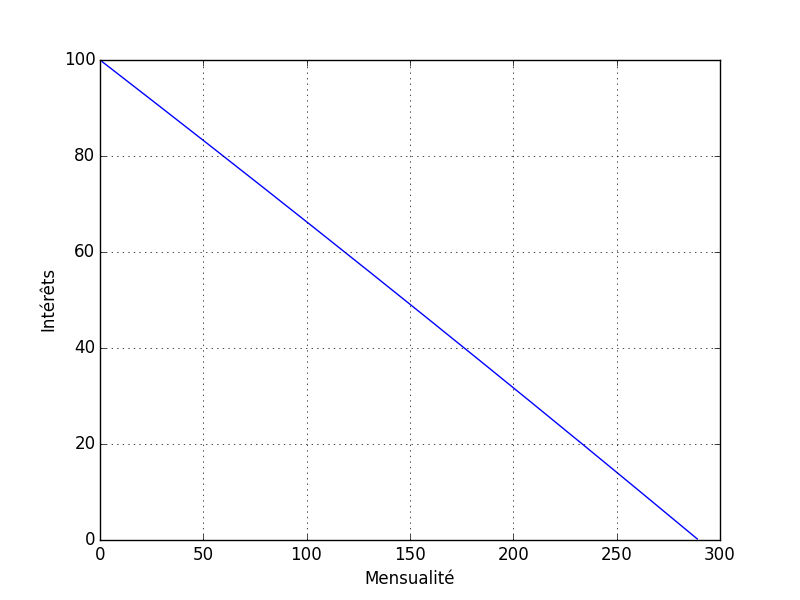
\includegraphics[width=0.5\textwidth]{interets.png}
\end{tabular}
\end{center}